\documentclass[a4paper, 14pt]{extarticle}
\usepackage[settings]{markdown}
\usepackage{minted}

% Поля
%--------------------------------------
\usepackage{geometry}
\geometry{a4paper,tmargin=2cm,bmargin=2cm,lmargin=3cm,rmargin=1cm}
%--------------------------------------


%Russian-specific packages
%--------------------------------------
\usepackage[T2A]{fontenc}
\usepackage[utf8]{inputenc} 
\usepackage[english, main=russian]{babel}
%--------------------------------------

\usepackage{textcomp}

% Красная строка
%--------------------------------------
\usepackage{indentfirst}               
%--------------------------------------             


%Graphics
%--------------------------------------
\usepackage{graphicx}
\graphicspath{ {./images/} }
\usepackage{wrapfig}
%--------------------------------------

% Полуторный интервал
%--------------------------------------
\linespread{1.3}                    
%--------------------------------------

%Выравнивание и переносы
%--------------------------------------
% Избавляемся от переполнений
\sloppy
% Запрещаем разрыв страницы после первой строки абзаца
\clubpenalty=10000
% Запрещаем разрыв страницы после последней строки абзаца
\widowpenalty=10000
%--------------------------------------

%Списки
\usepackage{enumitem}

%Подписи
\usepackage{caption} 

%Гиперссылки
\usepackage{hyperref}

\hypersetup {
	unicode=true
}

%Рисунки
%--------------------------------------
\DeclareCaptionLabelSeparator*{emdash}{~--- }
\captionsetup[figure]{labelsep=emdash,font=onehalfspacing,position=bottom}
%--------------------------------------

\usepackage{tempora}
\usepackage{amsmath}
\usepackage{color}
\usepackage{listings}
\lstset{
  belowcaptionskip=1\baselineskip,
  breaklines=true,
  frame=L,
  xleftmargin=\parindent,
  language=Python,
  showstringspaces=false,
  basicstyle=\footnotesize\ttfamily,
  keywordstyle=\bfseries\color{blue},
  commentstyle=\itshape\color{purple},
  identifierstyle=\color{black},
  stringstyle=\color{red},
}

%--------------------------------------
%			НАЧАЛО ДОКУМЕНТА
%--------------------------------------

\begin{document}

%--------------------------------------
%			ТИТУЛЬНЫЙ ЛИСТ
%--------------------------------------
\begin{titlepage}
\thispagestyle{empty}
\newpage


%Шапка титульного листа
%--------------------------------------
\vspace*{-60pt}
\hspace{-65pt}
\begin{minipage}{0.3\textwidth}
\hspace*{-20pt}\centering

\includegraphics[width=\textwidth]{emblem}
\end{minipage}
\begin{minipage}{0.67\textwidth}\small \textbf{
\vspace*{-0.7ex}
\hspace*{-6pt}\centerline{Министерство науки и высшего образования Российской Федерации}
\vspace*{-0.7ex}
\centerline{Федеральное государственное бюджетное образовательное учреждение }
\vspace*{-0.7ex}
\centerline{высшего образования}
\vspace*{-0.7ex}
\centerline{<<Московский государственный технический университет}
\vspace*{-0.7ex}
\centerline{имени Н.Э. Баумана}
\vspace*{-0.7ex}
\centerline{(национальный исследовательский университет)>>}
\vspace*{-0.7ex}
\centerline{(МГТУ им. Н.Э. Баумана)}}
\end{minipage}
%--------------------------------------

%Полосы
%--------------------------------------
\vspace{-25pt}
\hspace{-35pt}\rule{\textwidth}{2.3pt}

\vspace*{-20.3pt}
\hspace{-35pt}\rule{\textwidth}{0.4pt}
%--------------------------------------

\vspace{1.5ex}
\hspace{-35pt} \noindent \small ФАКУЛЬТЕТ\hspace{50pt} <<Информатика и системы управления>>

\vspace*{-16pt}
\hspace{47pt}\rule{0.83\textwidth}{0.4pt}

\vspace{0.5ex}
\hspace{-35pt} \noindent \small КАФЕДРА\hspace{50pt} <<Теоретическая информатика и компьютерные технологии>>

\vspace*{-16pt}
\hspace{30pt}\rule{0.866\textwidth}{0.4pt}
  
\vspace{11em}

\begin{center}
\Large {\bf Лабораторная работа № 5\_1} \\ 
\large {\bf по курсу <<Распределение параллельных и распределённых программ>>}\\
\large <<Синхронизация потоков>>
\end{center}\normalsize

\vspace{8em}


\begin{flushright}
  {Студент группы ИУ9-51Б Горбунов А. Д.\hspace*{15pt} \\
  \vspace{2ex}
  Преподаватель Царёв А. С.\hspace*{15pt}}
\end{flushright}

\bigskip

\vfill
 

\begin{center}
\textsl{Москва 2024}
\end{center}
\end{titlepage}
%--------------------------------------
%		КОНЕЦ ТИТУЛЬНОГО ЛИСТА
%--------------------------------------

\renewcommand{\ttdefault}{pcr}

\setlength{\tabcolsep}{3pt}
\newpage
\setcounter{page}{2}

\section{Задача}\label{Sect::task}
\par
    Использование барьерной синхронизации - задача "эволюция". Дан двумерный массив клеток, каждая из которых либо содержит организм (1), либо пуста (0), изначально он заполняется случайными значениями. Каждая клетка проверяет состояние своих соседей (их 8) и изменяет своё по правилам:

    \begin{itemize}
        \item Живая клетка, вокруг которой < 2 живых клеток, умирает от одиночества.
        \item Живая клетка, вокруг которой есть 2 или 3 живых клеток, выживает.
        \item Живая клетка, вокруг которой > 3 живых клеток, умирает от перенаселения.
        \item Пустая клетка, рядом с которой равно 3 живых соседа, оживает.
    \end{itemize}

    
    Реализовать заданное количество шагов моделирования при помощи n потоков. Каждый поток должен вычислить значения в заданной ему полосе матрицы. На каждом шаге результат моделирования необходимо записывать в новую матрицу. По окончании очередного шага необходимо скопировать содержимое новой матрицы в исходную. Шаги между потоками синхронизировать с помощью барьера (ни один из потоков не должен начинать следующий шаг, пока все не закончили текущий). Учесть следующие моменты:

    
    \begin{itemize}
        \item у клеток, находящихся на первой строке, первом столбце, последней строке и последнем столбце, соседями являются клетки с противоположной стороны матрицы
        \item каждый поток видит только свою часть матрицы, поэтому если ему необходим элемент, которого в его части матрицы нет, он должен каким-либо образом составлять запрос на то, чтобы тот поток, в котором этот элемент есть, его ему предоставил.
    \end{itemize}

    
    Замерить среднее время выполнения одного шага алгоритма и сравнить со средним временем выполнения одного шага без использования потоков. 

    
    Результат внести в отчёт.


\section{Код решения}
\begin{minted}{c++}
                                        Файл main.cpp:
#include <iostream>
#include <vector>
#include <thread>
#include <chrono>
#include <cstdlib>
#include <ctime>

using namespace std;

void initMatrix(vector<vector<int>>& matrix, int rows, int cols) {
    for (int i = 0; i < rows; i++) 
        for (int j = 0; j < cols; j++) 
            matrix[i][j] = rand() % 2;
}

int countLiveNeighbors(const vector<vector<int>>& matrix, int rows, int cols, int x, int y) {
    int count = 0;
    for (int i = -1; i <= 1; i++) 
        for (int j = -1; j <= 1; j++) {
            if (i == 0 && j == 0) continue;
            int nx = (x + i + rows) % rows;
            int ny = (y + j + cols) % cols;
            count += matrix[nx][ny];
        }
    return count;
}

void evolveStep(const vector<vector<int>>& currentMatrix, vector<vector<int>>& nextMatrix, int rows, int cols, int startRow, int endRow) {
    for (int i = startRow; i < endRow; ++i) 
        for (int j = 0; j < cols; ++j) {
            int liveNeighbors = countLiveNeighbors(currentMatrix, rows, cols, i, j);
            if (currentMatrix[i][j] == 1) {
                if (liveNeighbors < 2 || liveNeighbors > 3) 
                    nextMatrix[i][j] = 0;
                
            } else 
                if (liveNeighbors == 3) 
                    nextMatrix[i][j] = 1;  
        }
}

void evolveStepWithThreads(vector<vector<int>>& currentMatrix, vector<vector<int>>& nextMatrix, int rows, int cols, int numThreads) {
    vector<thread> threads;
    int chunkSize = rows / numThreads;

    for (int i = 0; i < numThreads; ++i) {
        int startRow = i * chunkSize;
        int endRow = (i == numThreads - 1) ? rows : (i + 1) * chunkSize;
        threads.emplace_back(evolveStep, ref(currentMatrix), ref(nextMatrix), rows, cols, startRow, endRow);
    }

    for (auto& t : threads)
        t.join();
}

void threadMain(vector<vector<int>>& currentMatrix, vector<vector<int>>& nextMatrix, int rows, int cols, int numSteps, int numThreads) {
    initMatrix(currentMatrix, rows, cols);

    auto start = chrono::high_resolution_clock::now();

    for (int step = 0; step < numSteps; ++step) {
        evolveStepWithThreads(currentMatrix, nextMatrix, rows, cols, numThreads);
        currentMatrix = nextMatrix;
    }

    auto end = chrono::high_resolution_clock::now();
    chrono::duration<double> duration = end - start;
    cout << "Среднее время выполнения с "<< numThreads <<" потоками: " << duration.count() / numSteps  << " секунд" << endl;
}

int main() {
    srand(time(0));

    int rows = 10000;
    int cols = 10000;
    int numSteps = 100;

    vector<vector<int>> currentMatrix(rows, vector<int>(cols));
    vector<vector<int>> nextMatrix(rows, vector<int>(cols));

    threadMain(currentMatrix, nextMatrix, rows, cols, numSteps, 2);
    threadMain(currentMatrix, nextMatrix, rows, cols, numSteps, 4);
    threadMain(currentMatrix, nextMatrix, rows, cols, numSteps, 6);
    threadMain(currentMatrix, nextMatrix, rows, cols, numSteps, 8);
    threadMain(currentMatrix, nextMatrix, rows, cols, numSteps, 10);
    threadMain(currentMatrix, nextMatrix, rows, cols, numSteps, 12);
    threadMain(currentMatrix, nextMatrix, rows, cols, numSteps, 14);
    threadMain(currentMatrix, nextMatrix, rows, cols, numSteps, 16);

    initMatrix(currentMatrix, rows, cols);

    auto start = chrono::high_resolution_clock::now();

    for (int step = 0; step < numSteps; ++step) {
        evolveStep(currentMatrix, nextMatrix, rows, cols, 0, rows);
        currentMatrix = nextMatrix;
    }

    auto end = chrono::high_resolution_clock::now();
    chrono::duration<double> duration = end - start;
    cout << "Среднее ремя выполнения без потоков: " << duration.count() / numSteps  << " секунд" << endl;

    return 0;
}

\end{minted}

\section{Результат запуска}
    
\begin{figure}[H]
	\centering
	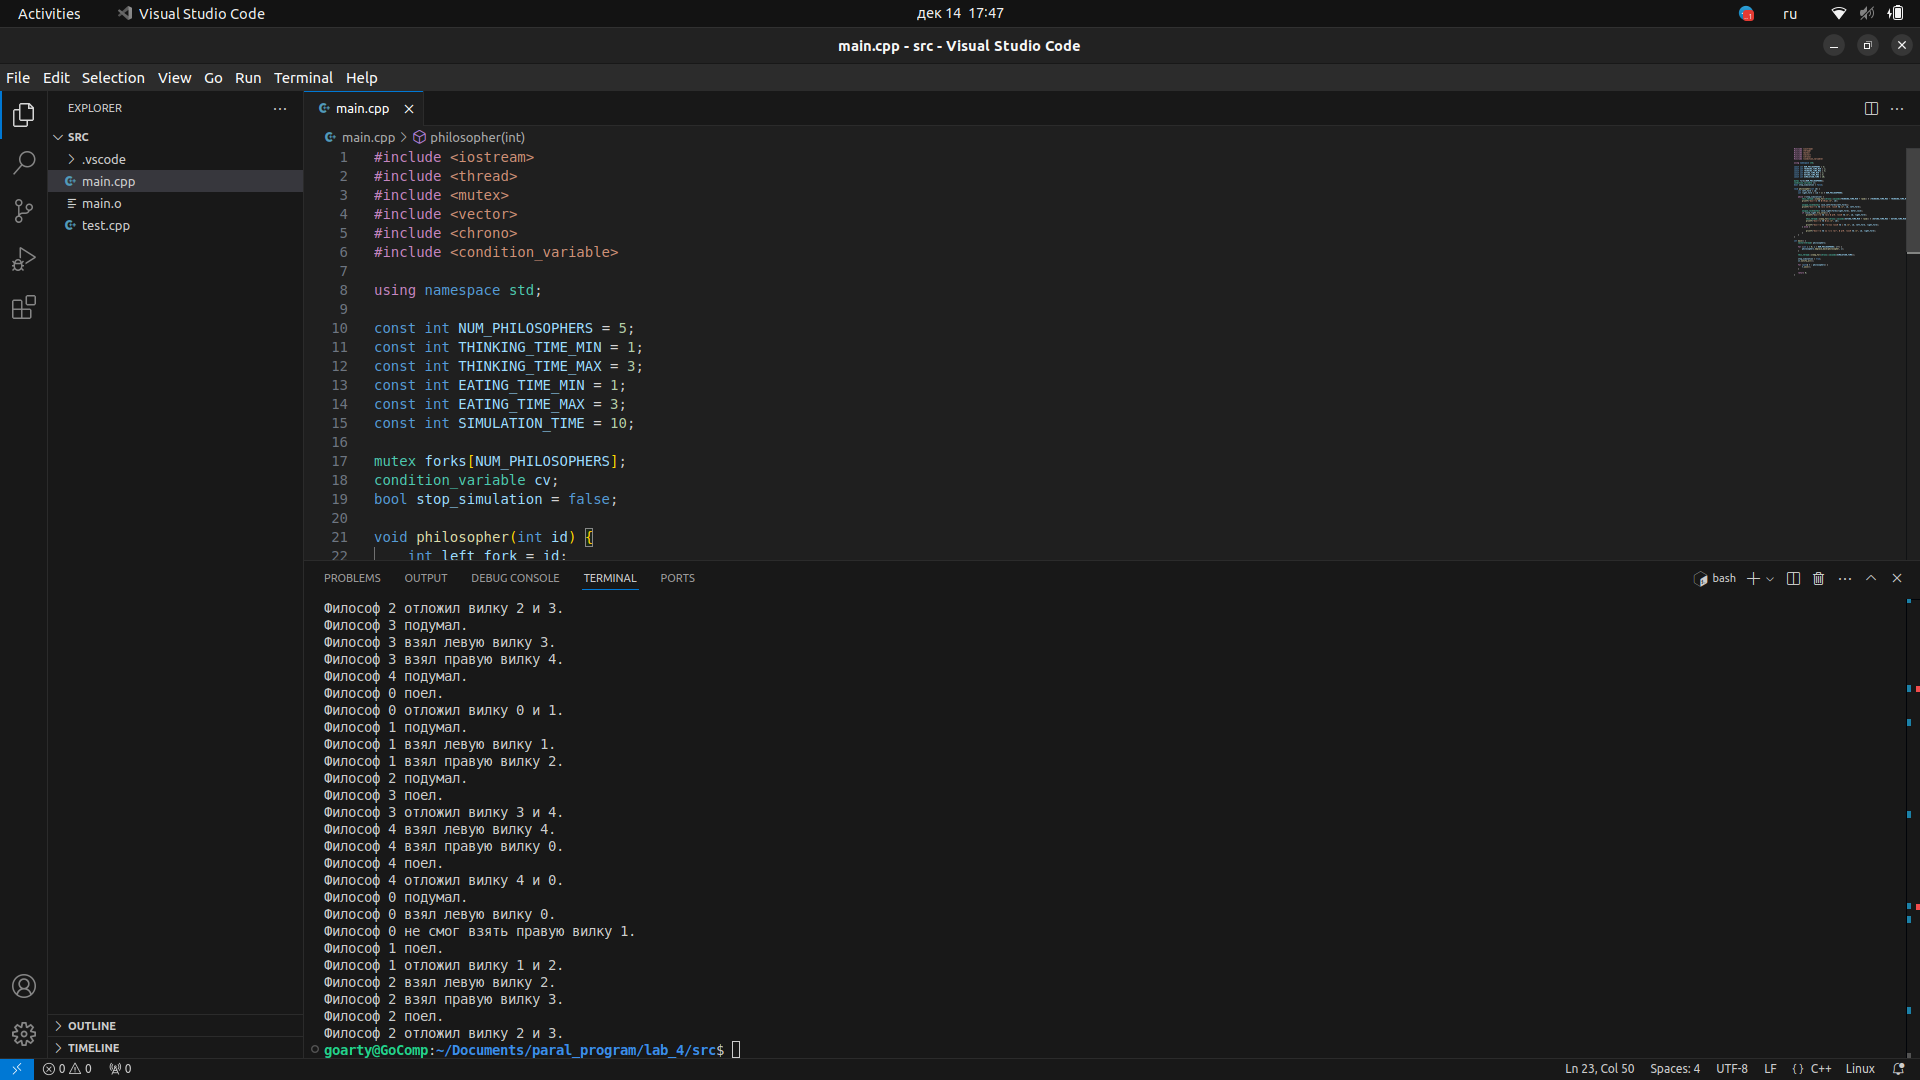
\includegraphics[width=0.8\textwidth]{picture.png}
\label{fig:picture.png}
\end{figure}

\section{График}
    
\begin{figure}[H]
	\centering
	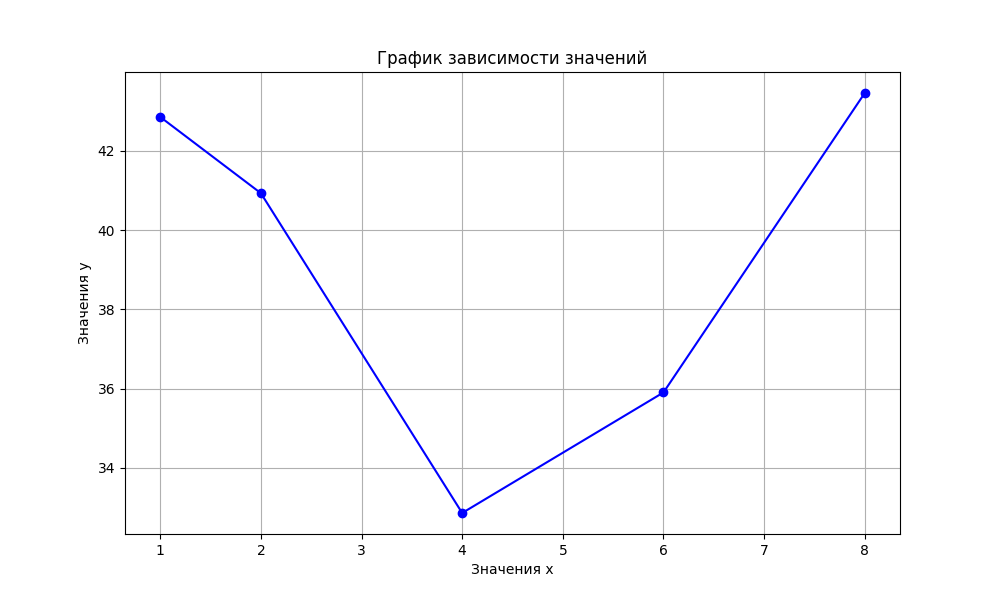
\includegraphics[width=0.8\textwidth]{graph.png}
\label{fig:picture.png}
\end{figure}

\section{Заключение}

    Из результата работы программы с потоками и без с размером квадратной матрицы 10000 и количеством шагов моделирования равном 100 можно понять что использование потоков в разы ускаряют выполнение данной программы.

\end{document}

